%%%%%%%%%%%%%%%%%%%%%%%%%%%%%%%%%%%%%%%%%
% Beamer Presentation
% LaTeX Template
% Version 1.0 (10/11/12)
%
% This template has been downloaded from:
% http://www.LaTeXTemplates.com
%
% License:
% CC BY-NC-SA 3.0 (http://creativecommons.org/licenses/by-nc-sa/3.0/)
%
%%%%%%%%%%%%%%%%%%%%%%%%%%%%%%%%%%%%%%%%%

%----------------------------------------------------------------------------------------
%	PACKAGES AND THEMES
%----------------------------------------------------------------------------------------

\documentclass[xcolor=svgnames]{beamer}

\mode<presentation> {

% The Beamer class comes with a number of default slide themes
% which change the colors and layouts of slides. Below this is a list
% of all the themes, uncomment each in turn to see what they look like.

% \usetheme{default}
% \usetheme{AnnArbor}
% \usetheme{Antibes}
%\usetheme{Bergen}
% \usetheme{Berkeley}
% \usetheme{Berlin}
\usetheme{Boadilla}
% \usetheme{CambridgeUS}
% \usetheme{Copenhagen}
% \usetheme{Darmstadt}
% \usetheme{Dresden}
% \usetheme{Frankfurt}
% \usetheme{Goettingen}
% \usetheme{Hannover}
% \usetheme{Ilmenau}
% \usetheme{JuanLesPins}
% \usetheme{Luebeck}
% \usetheme{Madrid}
% \usetheme{Malmoe}
% \usetheme{Marburg}
% \usetheme{Montpellier}
% \usetheme{PaloAlto}
% \usetheme{Pittsburgh}
% \usetheme{Rochester}
% \usetheme{Singapore}
% \usetheme{Szeged}
% \usetheme{Warsaw}

% As well as themes, the Beamer class has a number of color themes
% for any slide theme. Uncomment each of these in turn to see how it
% changes the colors of your current slide theme.

% \usecolortheme{albatross}
% \usecolortheme{beaver}
%\usecolortheme{beetle}
% \usecolortheme{crane}
%  \usecolortheme{dolphin}
% \usecolortheme{dove}
% \usecolortheme{fly}
% \usecolortheme{lily}
% \usecolortheme{orchid}
% \usecolortheme{rose}
% \usecolortheme{seagull}
% \usecolortheme{seahorse}
% \usecolortheme{whale}
% \usecolortheme{wolverine}

% \setbeamertemplate{footline} % To remove the footer line in all slides uncomment this line
%\setbeamertemplate{footline}[page number] % To replace the footer line in all slides with a simple slide count uncomment this line

% \setbeamertemplate{navigation symbols}{} % To remove the navigation symbols from the bottom of all slides uncomment this line
}

\usepackage{graphicx} % Allows including images
\usepackage{booktabs} % Allows the use of \toprule, \midrule and \bottomrule in tables
\usepackage{hyperref}
\usepackage{tikz}

\addtobeamertemplate{frametitle}{}{%
\begin{tikzpicture}[remember picture,overlay]
\node[anchor=north east,yshift=2pt] at (current page.north east) {\includegraphics[height=0.8cm]{iiit-new.png}};
\end{tikzpicture}}

\setbeamercolor{title in head/foot}{bg=OrangeRed, fg=White}
\setbeamercolor{author in head/foot}{bg=RoyalBlue, fg=White}
\setbeamercolor{date in head/foot}{bg=SlateGray, fg=White}

%----------------------------------------------------------------------------------------
%	TITLE PAGE
%----------------------------------------------------------------------------------------

\title[Discrete Structures]{Discrete Structures} % The short title appears at the bottom of every slide, the full title is only on the title page
\author{IIIT Hyderabad} % Your name
\institute[] % Your institution as it will appear on the bottom of every slide, may be shorthand to save space
{
Monsoon 2020 \\ % Your institution for the title page
\medskip
\textit{Tutorial 1 Solutions} % Your email address
}
\date{September 18, 2020} % Date, can be changed to a custom date

\begin{document}

\begin{frame}
\titlepage % Print the title page as the first slide
\end{frame}

\begin{frame}
\frametitle{Introduction} % Table of contents slide, comment this block out to remove it
\tableofcontents % Throughout your presentation, if you choose to use \section{} and \subsection{} commands, these will automatically be printed on this slide as an overview of your presentation
\end{frame}

%----------------------------------------------------------------------------------------
%	PRESENTATION SLIDES
%----------------------------------------------------------------------------------------

%------------------------------------------------
\section{Questions}
%------------------------------------------------


%------------------------------------------------
\subsection{Question 1}
%------------------------------------------------
\begin{frame}
\frametitle{Question 1}

\textbf{1.1}. Find the power set (or $\mathcal{P}(S)$) and it's order (or $|\mathcal{P}(S)|$) for the following sets - 
\begin{itemize}
    \item Set $S$ = \{$\phi$\}
    \\ \textbf{\underline{Sol:}} $\mathcal{P}(S)$ = \big\{$\phi$,\{$\phi$\}\big\}, $|\mathcal{P}(S)|$ = 2
    \item Set $S$ = \{a\}
    \\ \textbf{\underline{Sol:}} $\mathcal{P}(S)$ = \big\{$\phi$,\{a\}\big\}, $|\mathcal{P}(S)|$ = 2
    \item Set $S$ = \{a, $\phi$\}
    \\ \textbf{\underline{Sol:}} $\mathcal{P}(S)$ = \Big\{$\phi$,\{a\},\{$\phi$\},\{a, $\phi$\}\Big\}, $|\mathcal{P}(S)|$ = 4
    \item Set $S$ = \{a, \{$\phi$\}\}
    \\ \textbf{\underline{Sol:}} $\mathcal{P}(S)$ = \Big\{$\phi$,\{a\},\big\{\{$\phi$\}\big\},\big\{a, \{$\phi$\}\big\}\Big\}, $|\mathcal{P}(S)|$ = 4
    \item Set $S$ = \{$\phi$, \{$\phi$\}, \{\{$\phi$\}\}\} 
    \\ \textbf{\underline{Sol:}} $\mathcal{P}(S)$ = \Big\{$\phi$, \{$\phi$\}, \big\{\{$\phi$\}\big\}, \big\{\big\{\{$\phi$\}\big\}\big\}, \\ 
    \hspace{2.3cm} \big\{$\phi$,\{$\phi$\}\big\} ,\big\{$\phi$,\{\{$\phi$\}\}\big\},
    \big\{$\phi$,\{\{$\phi$\}\}\big\}, \\
    \hspace{2.3cm} \big\{$\phi$, \{$\phi$\},\{\{$\phi$\}\}\big\}\Big\}, $|\mathcal{P}(S)|$ = 8\end{itemize}
\vspace{3mm}
\end{frame}
\begin{frame}{Question 1}
\textbf{1.2}. If $|A|$ = $m$ and $|B|$ = $n$ and $A$ and $B$ are not mutually disjoint. Let
\begin{align*}
\mathcal{P}_i(S) = \mathcal{P}(\mathcal{P}(\mathcal{P}\ldots \mathcal{P}(S)))) \text{  \textit{i}}  \text{    times}
\end{align*}
 (Given m $\geq$ n)
  then what are the bounds of the value of $|\mathcal{P}_4(A-B)|$, $| \mathcal{P}_2(A-B)|$.
  
  *[ On the basis of above, can you tell about $|\mathcal{P}_4(A-B) - \mathcal{P}_2(A-B)|$? ]
  \textbf{\underline{Sol:}} 
  We have that $A - B &= A - (A \cap B)$.  Now $A \cap B$ can have maximum $n$ and minimum $1$ elements (since not disjoint). Thus 
  \begin{align*}
      m - n \leq |A - (A \cap B)| \leq m - 1 \\
      2^{m-n} \leq |P(A - (A \cap B))| \leq 2^{m-1} \\
      2^{2^{m - n}} \leq |P_2(A - (A \cap B))| \leq 2^{2^{m-1}} \\
      \vdots \\
      2^{2^{2^{2^{m-n}}}} \leq |P_4(A - (A \cap B))| \leq 2^{2^{2^{2^{m-1}}}}
  \end{align*}
\end{frame}



%------------------------------------------------
\subsection{Question 2}
%------------------------------------------------
\begin{frame}
\frametitle{Question 2}

For answering this question, go to:
\href{https://tinyurl.com/dstut1}{\underline{tinyurl.com/dstut1}}

\vspace{5mm}

True or False:

\begin{enumerate}
    \item $\phi \subseteq \{\phi\}$ -  \textbf{True}
    \item $\{x^2|x^2 = 1\} = \{x|x^2 = x\}$  - \textbf{False} \\
    \item $\mathcal{P}(\{x, y, \{x\}, \{y\}) = \mathcal{P}(\{x, y, \{x, y\})$  -             \textbf{False} 
    \item $\{a, \phi\} \in \{a\}$ -  \textbf{False}
    \item $\{a, \phi\} \subseteq \{a, \{a, \phi\}\}$ - \textbf{False}
    \item If $a \in \mathcal{P}(A)$, then $a \in A$ always - \textbf{False}
    \item For any set $A$, $A \subseteq A$ - \textbf{True}
    \item For any set $A$, $A \in A$ - \textbf{False}
    \item Every nonempty set has at least two subsets - \textbf{True}
\end{enumerate}
\end{frame}


\begin{frame}
\frametitle{Question 2 explanations}

True or False:

\begin{enumerate}
    \item \textbf{\underline{Sol:}} $\subseteq$ means "subset of", and $\phi$ is a subset of every set.
    \item \textbf{\underline{Sol:}} LHS describes the set \{1\}. RHS describes the set \{0,1\}. 
    \item \textbf{\underline{Sol:}} The cardinality of both the setsitself is different.
    \item \textbf{\underline{Sol:}} $\phi \notin \{a\}$. However $\phi \subseteq \{a\}$. 
    \item \textbf{\underline{Sol:}} $\phi \notin \{a, \{a, \phi\}\}$
    \item \textbf{\underline{Sol:}} Take $A = \{4\}$. $\mathcal{P}(A) = \{\phi, \{4\}\}$, now both $\phi \notin A$ and $\{4\} \notin A$
    \item \textbf{\underline{Sol:}} Take any arbitrary set $A$. Now by the definition of subset for $A \subseteq A$ : $\forall x \in A,\ x \in A$ | which is always \textbf{true} 
    \item \textbf{\underline{Sol:}} This is not always true. Set S = \{a\}, \{a\} $\notin$ \{a\}
    \item \textbf{\underline{Sol:}} Power set of a set S with cardinality $|S|$ has $2^{|S|}$ elements, and thus this is true.
\end{enumerate}
\end{frame}

%------------------------------------------------
\subsection{Question 3}
%------------------------------------------------
\begin{frame}
\frametitle{Question 3}
\textbf{3.1} Given $A = \{a, b, \{a, c\}, \phi \}$. Determine the following:
\begin{itemize}
    \item $A - \phi$ \\
    \textbf{\underline{Sol:}} $A - \phi = A$
    \item $A - \{a, c\}$ \\ 
    \textbf{\underline{Sol:}} $A - \{a, c\} = \{b, \{a, c \}, \phi\}$
    \item $A - \{\{a, c\}\}$ \\
    \textbf{\underline{Sol:}} $A - \{\{a, c\}\} = \{a, b, \phi\}$
    \item $\{a, c\} - A$ \\
    \textbf{\underline{Sol:}} $\{a,c\} - A = \{c\}$
\end{itemize}
\end{frame}
\begin{frame}
\frametitle{Question 3}
\textbf{3.2} One of the following set is different, which one ? (Choose one, MCQ)($\land$ is \textbf{AND} and $\lor$ is \textbf{OR})
\begin{enumerate}
    \item Set $S$ = $\{x |  (x^2 = 1 ) \lor (x^2 = 4) \lor (x \text{ is prime} < 10) \}$
    \item Set $S$ = $\{x| (x^2 = 4) \lor (x^2 = 1) \lor (x \text{ is odd} < 10)\}$
    \item Set $S$ = $\{x | (x < 9) \land (x > -3) \land ((x \text{ is odd}) \lor (x^2 = 4) )\}$
    \item Set $S$ = $\{ -2,-1,1,2,3,5,7 \}$
\end{enumerate}
\vspace{2mm}
\textbf{\underline{Sol:}} \textbf{Option 2} \\ Option 2 describes the set $\{-2, -1, 1, 2, 3, 5, 7, 9\}$ whereas all others describe the set $\{ -2,-1,1,2,3,5,7 \}$.
\end{frame}



%------------------------------------------------
\subsection{Question 4}
%------------------------------------------------
\begin{frame}
\frametitle{Question 4}
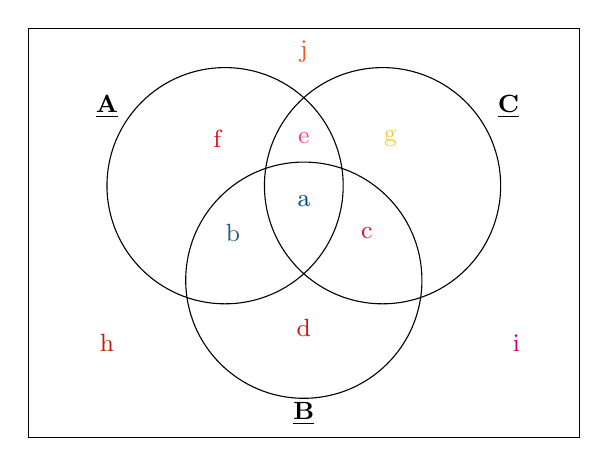
\begin{tikzpicture}
%% You can adjust the opacity here. For venn diagrams it is convenient to have a low opacity so that you can see intersections
	\begin{scope} [fill opacity = 1 ]
%% The draw command knows a lot of shapes. To make a rectangle you just need to specify two diagonal corners. Make sure you always have a semicolon at the end of your draw commands, otherwise latex flips out.
    \draw (-4,7) rectangle (3,1.8);
%% Similarly, you can make a circle by specifying the center and then the radius. You can also add a fill color, but if you're printing in black and white you'll probably want to remove that line.
    \draw (-1.5,5) circle (1.5);
    \draw (0.5,5) circle (1.5);
    \draw (-0.5,3.8) circle (1.5);
%% We can use the node command to label points. If you put your cursor on "LARGE" or "textbf" a box will drop down with size and text style options.
    \node [text={rgb,255:red,0; green,69; blue,135}] at (-0.5,4.8) {\small{a}};
    \node [text={rgb,255:red,37; green,97; blue,124}] at (-1.4,4.4) {\small{b}};
    \node [text={rgb,255:red,225; green,18; blue,39}] at (0.3,4.4) {\small{c}};
    \node [text={rgb,255:red,219; green,19; blue,22}] at (-0.5,3.2) {\small{d}};
    \node [text={rgb,255:red,255; green,64; blue,129}] at (-0.5,5.6) {\small{e}};
    \node [text={rgb,255:red,221; green,18; blue,18}] at (-1.6,5.6) {\small{f}};
    \node [text={rgb,255:red,240; green,204; blue,60}] at (0.6,5.6) {\small{g}};
    \node [text={rgb,255:red,184; green,37; blue,6}] at (-3,3) {\small{h}};
    \node [text={rgb,255:red,197; green,0; blue,111}] at (2.2,3) {\small{i}};
    \node [text={rgb,255:red,247; green,84; blue,36}] at (-0.5,6.7) {\small{j}};
    \node [text=black] at (-3,6) {\small{\textbf{\underline{A}}}};
    \node [text=black] at (-0.5,2.1) {\small{\textbf{\underline{B}}}};
    \node [text=black]at (2.1,6) {\small{\textbf{\underline{C}}}};
    \end{scope}
%% And now you have a venn diagram. Yay!
%\draw[help lines](-5,5) grid (5,-6);    This line can draw the grid lines to help guide you. I use these when I'm writing the code and then delete this line when I publish the pdf.
\end{tikzpicture}
\\
\begin{enumerate}
    \item (U - (A $\cap$ B))' $\cup$ ((C - B) $\cap$ A') | \textbf{\underline{Sol:}} $\{a,b\} \cup \{g\}$ = $\{a,b,g\}$
    \item (A $\cap$ C') $\cup$ (A  $\cup$ B $\cup$ C )' | \textbf{\underline{Sol:}} $\{b,f\} \cup \{h,i, j\}$ = $\{b,f,h,i,j\}$
    \item (A - (B $\cap$ C)) $\cap$ (U' - (C $\cap$ B))' | \textbf{\underline{Sol:}} $\{b,e,f\} \cap \{U\}$  = $\{b,e,f\}$
\end{enumerate}
\end{frame}



\end{document} 